%versi 2 (8-10-2016)
\chapter{Landasan Teori}
\label{chap:teori}

Pada bab ini akan diuraikan teori-teori yang akan digunakan untuk pembangunan aplikasi ke analisis kota Bandung. Teori-teori tersebut adalah penjelasan tentang protokol HTTP, Penjelasan tentang \textit{JSOUP API}, Penjelasan tentang \textit{Google Direction API} dan teori JSON.

\section{Protokol HTTP}
\label{sec:protocolhttp} 

HTTP adalah protokol di balik World Wide Web. Dengan setiap transaksi web, HTTP dipanggil. HTTP adalah di balik setiap permintaan dokumen web atau grafis, setiap klik link hypertext, dan setiap penyerahan formulir. Web adalah tentang penyebaran informasi melalui Internet, dan HTTP adalah protokol yang digunakan untuk melakukannya.

\subsection{Transaksi HTTP}
\label{subsec:architecturehttp}

Berikut akan diilustrasikan transaksi web umum, menunjukkan HTTP yang dipertukarkan antara program \textit{client} dan \textit{program} server. \cite{wong2000http}:

\begin{itemize}
	\item berikut diberikan sebuah url : http:\/\/hypothetical.ora.com:80\/.
	\item Browser akan mengintepretasikan URL tersebut sebagai berikut :
			\begin{itemize}
				\item \(http:\/\/\) : menggunakan protokol HTTP.
				\item \(hypothetical.ora.com\) : menghubungi komputer melalui jaringan dengan hostname hypothetical.ora.com.
				\item \(:80\) : Terhubung ke komputer di port 80. Nomor port IP nomor dari 1 sampai 65535. Jika titik dua dan nomor port dihilangkan, nomor port diasumsikan nomor port \textit{default} HTTP, yang merupakan 80.
				\item \(\/\) : Apapun setelah nama host dan nomor port opsional dianggap sebagai jalan dokumen. Dalam ilustrasi ini, jalan dokumen adalah \/.
			\end{itemize}
			\item Pada ilustrasi ini browser menghubungkan ke hypothetical.ora.com pada port 80 menggunakan protokol HTTP. Pesan bahwa browser mengirimkan ke server adalah sebagai berikut:
			\begin{figure}[H]
				\centering		
				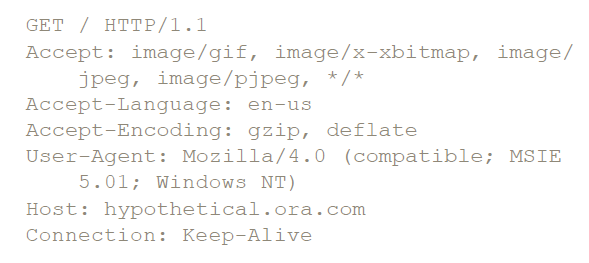
\includegraphics[scale=0.7]{Gambar/request.png}
				\caption[HTTP Request]{HTTP Request\cite{wong2000http}}
				\label{fig:httprequest}	
			\end{figure}
\end{itemize}

\section{JSOUP API}
\label{sec:jsoupapi}

JSOUP adalah sebuah \textit{library} java untuk bekerja dengan HTML dunia nyata.  JSOUP menyediakan API yang sangat nyaman untuk mengekstrak dan memanipulasi data, menggunakan DOM(Document Object Model) terbaik, CSS, dan metode yang mirip deengan jquery. JSOUP mengimplementasikan spesifikasi standar \textit{WHATWG HTML5} dan mengurai HTML menjadi DOM(Document Object Model) yang sama dengan peramban modern lakukan. JSOUP sendiri dirancang untuk menangani semua jenis HTML yang biasa ditemukan; dari yang murni dan memvalidasi, untuk tidak valid tag-soup; JSOUP akan membuat \textit{parsing tree} yang dapat dimengerti.

\subsection{Fungsi JSOUP}
\label{subsec:fungsijsoup}
berikut adalah fungsi dari JSOUP :
\begin{itemize}
	\item menghimpun dan mengurai HTML dari URL, file, atau \textsl{string}.
	\item mencari dan mengambil data, menggunakan \textit{DOM traversal} atau \textit{CSS selectors}.
	\item memanipulasi elemen HTML, atribut, dan teks.
	\item membersihkan konten yang dikirimkan pengguna terhadap daftar putih yang aman, untuk mencegah serangan XSS.
	\item memberi \textit{output} HTML yang rapi.
\end{itemize} 

\section{Google Direction API}
\label{subsec:googledirapi}

Google Maps Directions API adalah layanan yang menghitung arah antar lokasi menggunakan permintaan HTTP. Anda bisa mencari arah untuk beberapa moda transportasi, termasuk angkutan umum, mengemudi, berjalan atau bersepeda. Arah bisa menetapkan tempat asal, tujuan dan titik jalan baik sebagai string teks (misalnya "Chicago, IL" atau "Darwin, NT, Australia") atau sebagai koordinat garis lintang/garis bujur. Directions API bisa mengembalikan arah multi-bagian menggunakan serangkaian titik jalan. Layanan ini biasanya didesain untuk menghitung arah alamat statis (sudah diketahui sebelumnya) untuk penempatan konten aplikasi pada peta.

\subsection{Permintaan Arah}
\label{subsec:permintaanarahgoogledir}

Permintaan Google Maps Directions API mengambil bentuk berikut:

\url{https://maps.googleapis.com/maps/api/directions/output?parameters}

dalam hal ini, output bisa berupa salah satu nilai berikut: 
\begin{itemize}
	\item json (disarankan) menunjukkan output dalam JavaScript Object Notation (JSON).
	\item xml menunjukkan output berupa XML.
\end{itemize} 
Untuk mengakses Google Maps Directions API melalui HTTP, gunakan:

\url{http://maps.googleapis.com/maps/api/directions/output?parameters}

HTTP disarankan untuk aplikasi yang berisi data pengguna sensitif, seperti lokasi pengguna, dalam permintaan.

URL Google Maps Directions API dibatasi sekitar 2000 karakter, setelah Pengkodean URL. Karena sebagian URL Google Maps Directions API bisa melibatkan banyak lokasi sepanjang lintasan, berhati-hatilah dengan batas ini saat membangun URL Anda.

\subsection{Parameter Permintaan}
\label{subsec:parameterpermintaangoogledir}

Beberapa parameter tertentu diperlukan sementara yang lainnya bersifat opsional. Sebagaimana standar dalam URL, semua parameter dipisah menggunakan karakter ampersand (\&). Daftar parameter dan kemungkinan nilainya disebutkan di bawah ini.

\subsubsection{Parameter yang diperlukan}
\label{subsubsec:parameterwajib}
\begin{itemize}
	\item \textbf{origin} adalah alamat, nilai garis lintang/garis bujur tekstual, atau ID tempat asal yang ingin Anda hitung arahnya.
	\begin{itemize}
		\item Jika Anda meneruskan sebuah alamat sebagai string, layanan Directions akan melakukan geocode atas string itu dan mengubahnya menjadi koordinat garis lintang/garis bujur untuk menghitung arah. Koordinat ini mungkin berbeda dengan yang dikembalikan oleh Google Maps Geocoding API, misalnya pintu masuk bangunan dan bukan pusatnya.
		\item Jika Anda meneruskan koordinat, itu akan digunakan tanpa diubah untuk menghitung arah. Pastikan tidak ada spasi di antara nilai garis lintang dan garis bujur.
		\item ID Tempat harus diawali dengan \textbf{place\_id:}. ID tempat hanya bisa ditetapkan jika permintaan menyertakan kunci API atau ID klien Google Maps API for Work. Anda bisa mendapatkan ID tempat dari Google Maps Geocoding API dan Google Places API (termasuk Place Autocomplete).
	\end{itemize} 
	\item \textbf{destination} adalah alamat, nilai garis lintang/garis bujur tekstual, atau ID tempat tujuan yang ingin Anda hitung arahnya. Opsi untuk parameter destination sama dengan opsi untuk parameter origin yang dijelaskan di atas.
	\item \textbf{key} adalah kunci API aplikasi Anda. Kunci ini mengidentifikasi aplikasi Anda untuk keperluan manajemen kuota. 
\end{itemize} 

\subsubsection{Parameter yang diperlukan}
\label{subsubsec:parameteropsional}

\begin{itemize}
	\item \textbf{mode} (default-nya adalah driving) adalah menetapkan moda transportasi yang akan digunakan saat menghitung arah. 
	\item \textbf{waypoint} adalah menetapkan larik titik jalan. Titik jalan mengubah rute dengan mengarahkannya melalui lokasi yang ditetapkan. Titik jalan ditetapkan berupa koordinat garis lintang/garis bujur, ID tempat, atau alamat yang akan di-geocode. ID Tempat harus diawali dengan \textbf{place\_id:}. ID tempat hanya bisa ditetapkan jika permintaan menyertakan kunci API atau ID klien Google Maps API for Work. Titik jalan hanya didukung untuk arah mengemudi, berjalan dan bersepeda.
	\item \textbf{alternative} adalah jika diatur ke true, menetapkan bahwa layanan Directions mungkin menyediakan lebih dari satu rute alternatif dalam respons. Perhatikan, memberikan alternatif rute bisa meningkatkan waktu respons dari server.
	\item \textbf{avoid} adalah menunjukkan rute yang dihitung harus menghindari fitur yang ditandai. Parameter ini mendukung argumen berikut: 
	\begin{itemize}
		\item \textbf{tolls} menunjukkan rute yang dihitung harus menghindari jalan/jembatan tol.
		\item \textbf{highways} menunjukkan rute yang dihitung harus menghindari jalan raya.
		\item \textbf{ferries} menunjukkan rute yang dihitung harus menghindari penyeberangan feri.
		\item \textbf{indoor} menunjukkan rute yang dihitung harus menghindari tangga dalam ruangan untuk arah berjalan dan arah angkutan umum. Hanya permintaan yang menyertakan kunci API atau ID klien Google Maps API for Work yang akan menerima tangga dalam ruangan secara default.
	\end{itemize}
	\item \textbf{language} adalah menetapkan bahasa yang digunakan untuk mengembalikan hasil.
	\item \textbf{unit} adalah menetapkan sistem satuan yang akan digunakan saat menampilkan hasil.
	\item \textbf{region} adalah menetapkan kode wilayah, ditetapkan sebagai nilai yang berisi dua karakter ccTLD ("top-level domain").
	\item \textbf{arrival\_time} adalah menetapkan waktu kedatangan yang diinginkan untuk arah angkutan umum, dalam detik sejak tengah malam, 1 Januari 1970 UTC. Anda bisa menetapkan \textbf{departure\_time} atau \textbf{arrival\_time}, namun tidak boleh duanya.
	\item \textbf{departure\_time} adalah menetapkan waktu keberangkatan yang diinginkan. Anda bisa menetapkan waktu berupa integer dalam detik sejak tengah malam 1 Januari 1970 UTC. Atau, Anda bisa menetapkan nilai now, yang mengatur waktu keberangkatan ke waktu saat ini (dikoreksi ke detik terdekat). 
	\item \textbf{traffic\_model} (default-nya adalah \textbf{best\_guess}) adalah menetapkan asumsi yang akan digunakan saat menghitung waktu dalam lalu lintas. Pengaturan ini memengaruhi nilai yang dikembalikan di bidang \textbf{duration\_in\_traffic} dalam respons, yang berisi prediksi waktu dalam lalu lintas berdasarkan rata-rata historis. Parameter \textbf{traffic\_model} hanya bisa ditetapkan untuk arah mengemudi yang permintaannya menyertakan departure\_time, dan hanya jika permintaan menyertakan kunci API atau ID klien Google Maps API for Work.Nilai yang tersedia untuk parameter ini adalah: 
	\begin{itemize}
		\item \textbf{best\_guess} (default) menunjukkan \textbf{duration\_in\_traffic} yang dikembalikan harus berupa perkiraan waktu tempuh terbaik berdasarkan informasi riwayat kondisi lalu lintas dan lalu lintas saat ini. Lalu lintas saat ini menjadi kian penting bila \textbf{departure\_time} semakin dekat ke waktu sekarang.
		\item \textbf{pessimistic} menunjukkan \textbf{duration\_in\_traffic} yang dikembalikan lebih lama dari waktu tempuh sesungguhnya di hari-hari biasa, meskipun hari-hari tertentu dengan kondisi lalu lintas yang buruk mungkin melebihi nilai ini.
		\item \textbf{optimistic} menunjukkan \textbf{duration\_in\_traffic} yang dikembalikan harus lebih singkat dari waktu tempuh sesungguhnya di hari biasa, meskipun hari-hari tertentu dengan kondisi lalu lintas yang baik bisa lebih cepat dari nilai ini.
	\end{itemize}
	\item \textbf{transit\_mode} adalah menetapkan satu atau beberapa mode angkutan umum yang disukai. Parameter ini hanya bisa ditetapkan untuk arah angkutan umum, dan hanya jika permintaan menyertakan kunci API atau ID klien Google Maps API for Work. Parameter ini mendukung argumen berikut:
	\begin{itemize}
		\item \textbf{bus} menunjukkan rute yang sudah dihitung akan mengutamakan perjalanan dengan bus.
		\item \textbf{subway} menunjukkan rute yang sudah dihitung akan mengutamakan perjalanan dengan kereta bawah tanah.
		\item \textbf{train} menunjukkan rute yang sudah dihitung akan mengutamakan perjalanan dengan kereta api.
		\item \textbf{tram} menunjukkan rute yang sudah dihitung akan mengutamakan perjalanan dengan trem dan kereta ringan.
		\item \textbf{rail} menunjukkan rute yang sudah dihitung akan mengutamakan perjalanan dengan kereta api, trem, kereta ringan, dan kereta bawah tanah. Ini sama dengan \textbf{transit\_mode=train|tram|subway}.
	\end{itemize}
	\item \textbf{transit\_routing\_preference} adalah menetapkan preferensi untuk rute angkutan umum. Dengan parameter ini, Anda bisa mencondongkan opsi yang dikembalikan, bukannya menerima rute default terbaik yang dipilih oleh API. Parameter ini hanya bisa ditetapkan untuk arah angkutan umum, dan hanya jika permintaan menyertakan kunci API atau ID klien Google Maps API for Work. Parameter ini mendukung argumen berikut:
	\begin{itemize}
		\item \textbf{less\_walking} menunjukkan rute yang sudah dihitung akan mengutamakan jumlah berjalan kaki yang terbatas.
		\item \textbf{fewer\_transfers} menunjukkan rute yang sudah dihitung akan mengutamakan jumlah ganti angkutan yang terbatas.
	\end{itemize}
\end{itemize}

\section{JSON}
\label{sec:json}

JSON (JavaScript Object Notation) adalah format pertukaran data yang ringan, mudah dibaca dan ditulis oleh manusia, serta mudah diterjemahkan dan dibuat (generate) oleh komputer. Format ini dibuat berdasarkan bagian dari Bahasa Pemprograman JavaScript, Standar ECMA-262 Edisi ke-3 - Desember 1999. JSON merupakan format teks yang tidak bergantung pada bahasa pemprograman apapun karena menggunakan gaya bahasa yang umum digunakan oleh programmer keluarga C termasuk C, C++, C\#, Java, JavaScript, Perl, Python dll. Oleh karena sifat-sifat tersebut, menjadikan JSON ideal sebagai bahasa pertukaran-data.

\subsection{Struktur JSON}
\label{subsec:stukturjson}
JSON terbuat dari dua struktur :
\begin{itemize}
	\item Kumpulan pasangan nama/nilai.
	\item Daftar nilai terurutkan (an ordered list of values).
\end{itemize} 

Struktur-struktur data ini disebut sebagai struktur data universal. Pada dasarnya, semua bahasa pemprograman moderen mendukung struktur data ini dalam bentuk yang sama maupun berlainan. Hal ini pantas disebut demikian karena format data mudah dipertukarkan dengan bahasa-bahasa pemprograman yang juga berdasarkan pada struktur data ini.
 
\subsection{Bentuk-Bentuk JSON}
\label{subsec:bentukjson}
\begin{itemize}
	\item Objek
	Objek adalah sepasang nama/nilai yang tidak terurutkan. Objek dimulai dengan { (kurung kurawal buka) dan diakhiri dengan } (kurung kurawal tutup). Setiap nama diikuti dengan : (titik dua) dan setiap pasangan nama atau nilai dipisahkan oleh , (koma).
	\begin{figure}[H]
		\centering		
		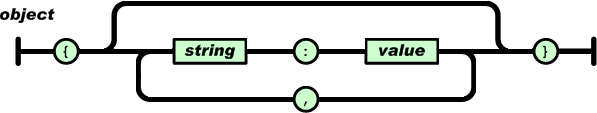
\includegraphics[scale=0.4]{Gambar/object.png}
		\caption[JSON Object]{JSON Object}
		\label{fig:jsonobject}	
	\end{figure}
	\item \textit{Array}
	\textit{Array} adalah kumpulan nilai yang terurutkan. Larik dimulai dengan [ (kurung kotak buka) dan diakhiri dengan ] (kurung kotak tutup). Setiap nilai dipisahkan oleh , (koma).
	\begin{figure}[H]
		\centering		
		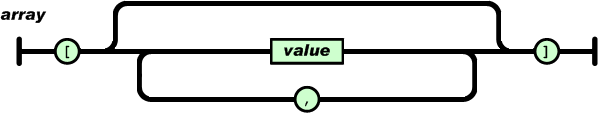
\includegraphics[scale=0.4]{Gambar/array.png}
		\caption[JSON Object]{JSON Array}
		\label{fig:jsonarray}	
	\end{figure}
\end{itemize} 

\subsection{Value JSON}
\label{subsec:bentukjson}
Nilai(\textit{value})dapat berupa sebuah string dalam tanda kutip ganda, atau angka, atau true atau false atau null, atau sebuah objek atau sebuah larik. Struktur-struktur tersebut dapat disusun bertingkat.
\begin{figure}[H]
	\centering		
	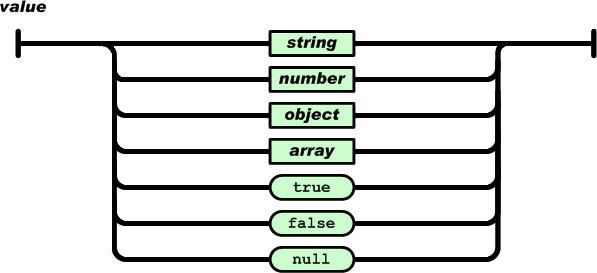
\includegraphics[scale=0.4]{Gambar/value.png}
	\caption[Value]{Value}
	\label{fig:value}	
\end{figure}

\subsubsection{\textit{String}}
\label{subsubsec:string}
String adalah kumpulan dari nol atau lebih karakter Unicode, yang dibungkus dengan tanda kutip ganda. Di dalam string dapat digunakan backslash escapes "\" untuk membentuk karakter khusus. Sebuah karakter mewakili karakter tunggal pada string. String sangat mirip dengan string C atau Java.

\begin{figure}[H]
	\centering		
	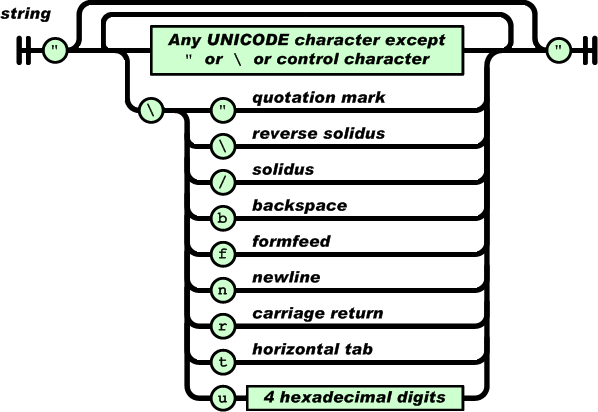
\includegraphics[scale=0.4]{Gambar/string.png}
	\caption[String]{String}
	\label{fig:string}	
\end{figure}

\subsubsection{Angka}
\label{subsubsec:Angka}
Angka adalah sangat mirip dengan angka di C atau Java, kecuali format oktal dan heksadesimal tidak digunakan.
\begin{figure}[H]
	\centering		
	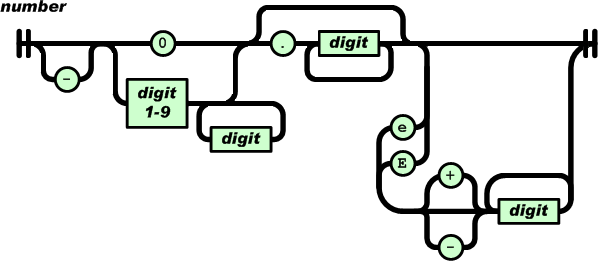
\includegraphics[scale=0.4]{Gambar/number.png}
	\caption[Angka]{Angka}
	\label{fig:number}	
\end{figure}